\documentclass[11pt]{article}

\usepackage{titling}
\usepackage{xcolor}
\usepackage{graphicx}
\usepackage{hyperref}
\hypersetup{%
  colorlinks=false,% hyperlinks will be black
  linkbordercolor=red,% hyperlink borders will be red
  pdfborderstyle={/S/U/W 1}% border style will be underline of width 1pt
}

\newcommand{\subtitle}[1]{%
  \posttitle{%
    \par\end{center}
    \begin{center}\large#1\end{center}
    \vskip0.5em}%
}

\begin{document}

\title{Applied Data Science Capstone Final Project}
\subtitle{Sports Facilities in Thessaloniki, Greece}
\author{Charalampos Kokkalis}
\maketitle 

\section{Introduction/Business Plan}
For the final project of the Applied Data Science Capstone, and since we were given the choice of our topic, I decided to do something related to my hometown, Thessaloniki, Greece, and to my main hobby, basketball (and sports in general). In the recent years, I have faced the challenge of finding proper sports facilities, in order to exercise, many times. Although there has been some movement in the market, there is still a great shortage of centers for sports, given the high demand due to the city being famous for its sports teams and thus motivating all its citizens to spend time trying different sports.

\section{Aim of the Analysis}
The aim of the following analysis is to find suggested sub-areas in the city of Thessaloniki where it would be worth building sports facilities. The outcome of this analysis would be useful both to the Municipality, which could make public sports facilities, and to individuals looking to start their own businesses in the market.

\section{Data Used}
\begin{itemize}
\item {To get access to a map of the city, I used the folium Python library.}
\item {To search for sports facilities in the area, I used the Foursquare API.}
\end{itemize}

\section{Methodology}
All the following steps can be found in the Jupyter Notebook (file name: Final Project.ipynb) in the \href{https://github.com/ckokkalis/Coursera_Capstone}{\color{blue} \underline {repository of the project}}.

\begin{enumerate}

\item To begin the analysis in the notebook we need to import the following libraries: 
\begin{figure}[htbp]
\centerline{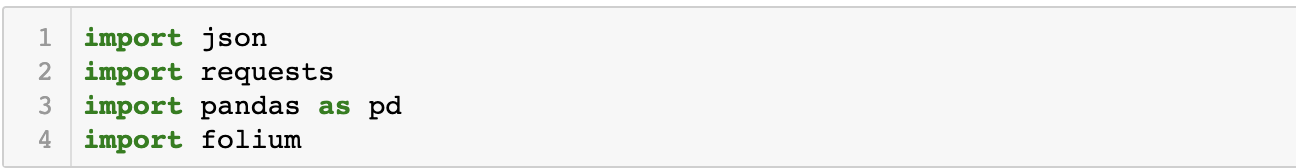
\includegraphics[scale=0.5]{libs.png}}
\end{figure}
\break json and requests are used to access the Foursquare API, pandas to store and access the data in Dataframes, and folium to display the resulting map.

\item We first make a request to the Foursquare API to get the data for Thessaloniki. The parameters show, including others, where the center of the area we are searching is located, what radius we want to consider, and what we are looking for in the area. Here, I had to use the Greek word for Sports Courts, since it gave more results due to most data being in Greek, making the analysis more meaningful and successful.
\begin{figure}[htbp]
\centerline{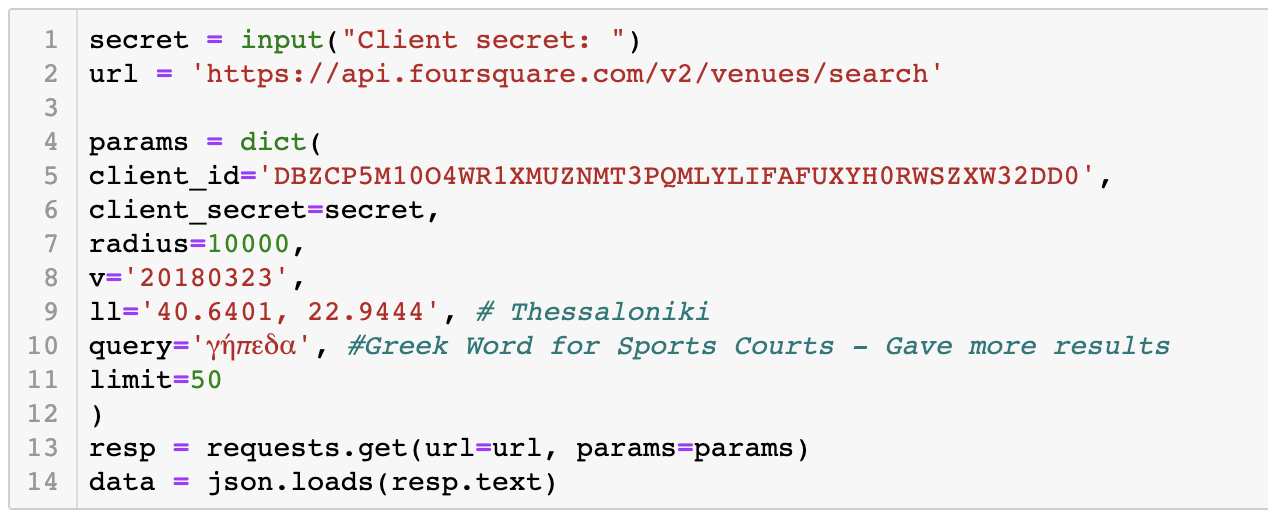
\includegraphics[scale=0.5]{1.png}}
\end{figure}
\pagebreak

\item From the data returned in the previous step, we access the list of venues. We display the head() of these to get an idea about what our data look like:
\begin{figure}[htbp]
\centerline{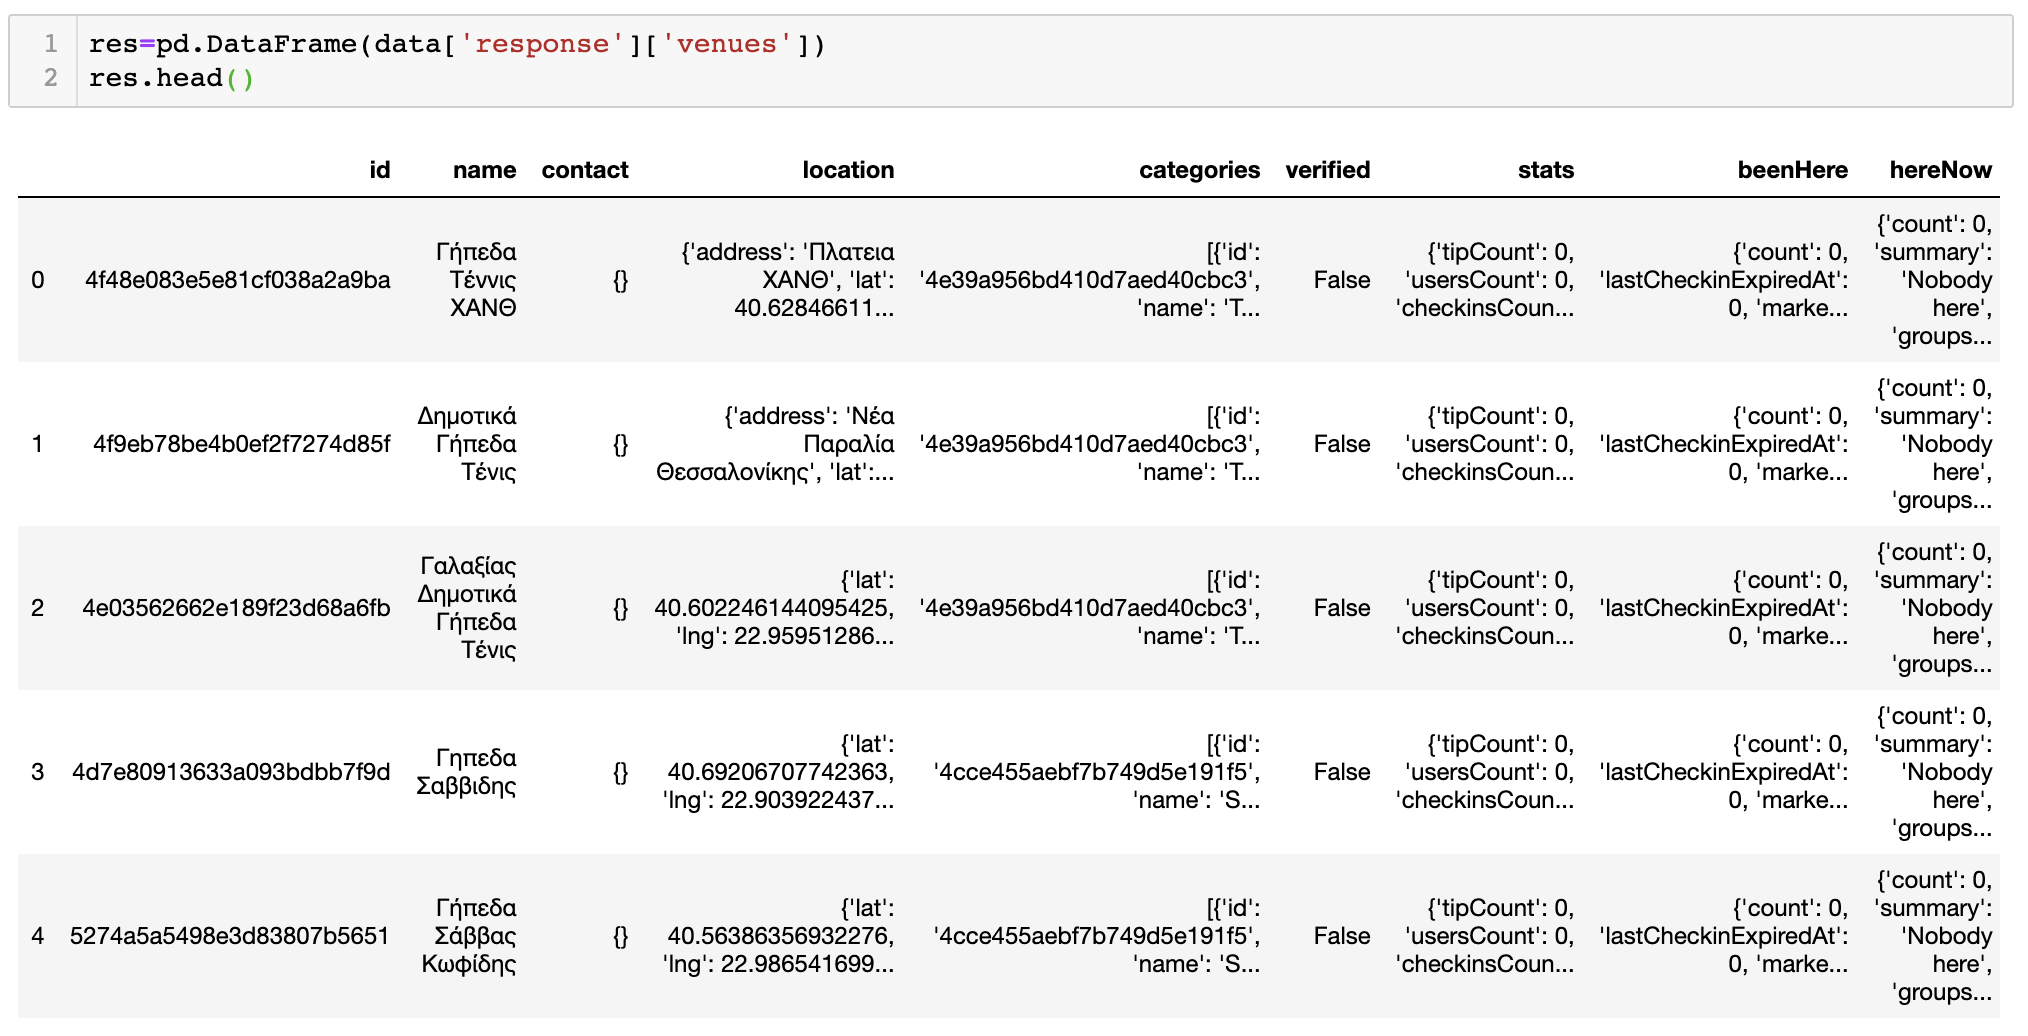
\includegraphics[scale=0.3]{2.png}}
\end{figure}

\item Finally, we access (using the folium Python library) the map of Thessaloniki, and add markers at all locations where we found sports centers. The result is the following: 
\begin{figure}[htbp]
\centerline{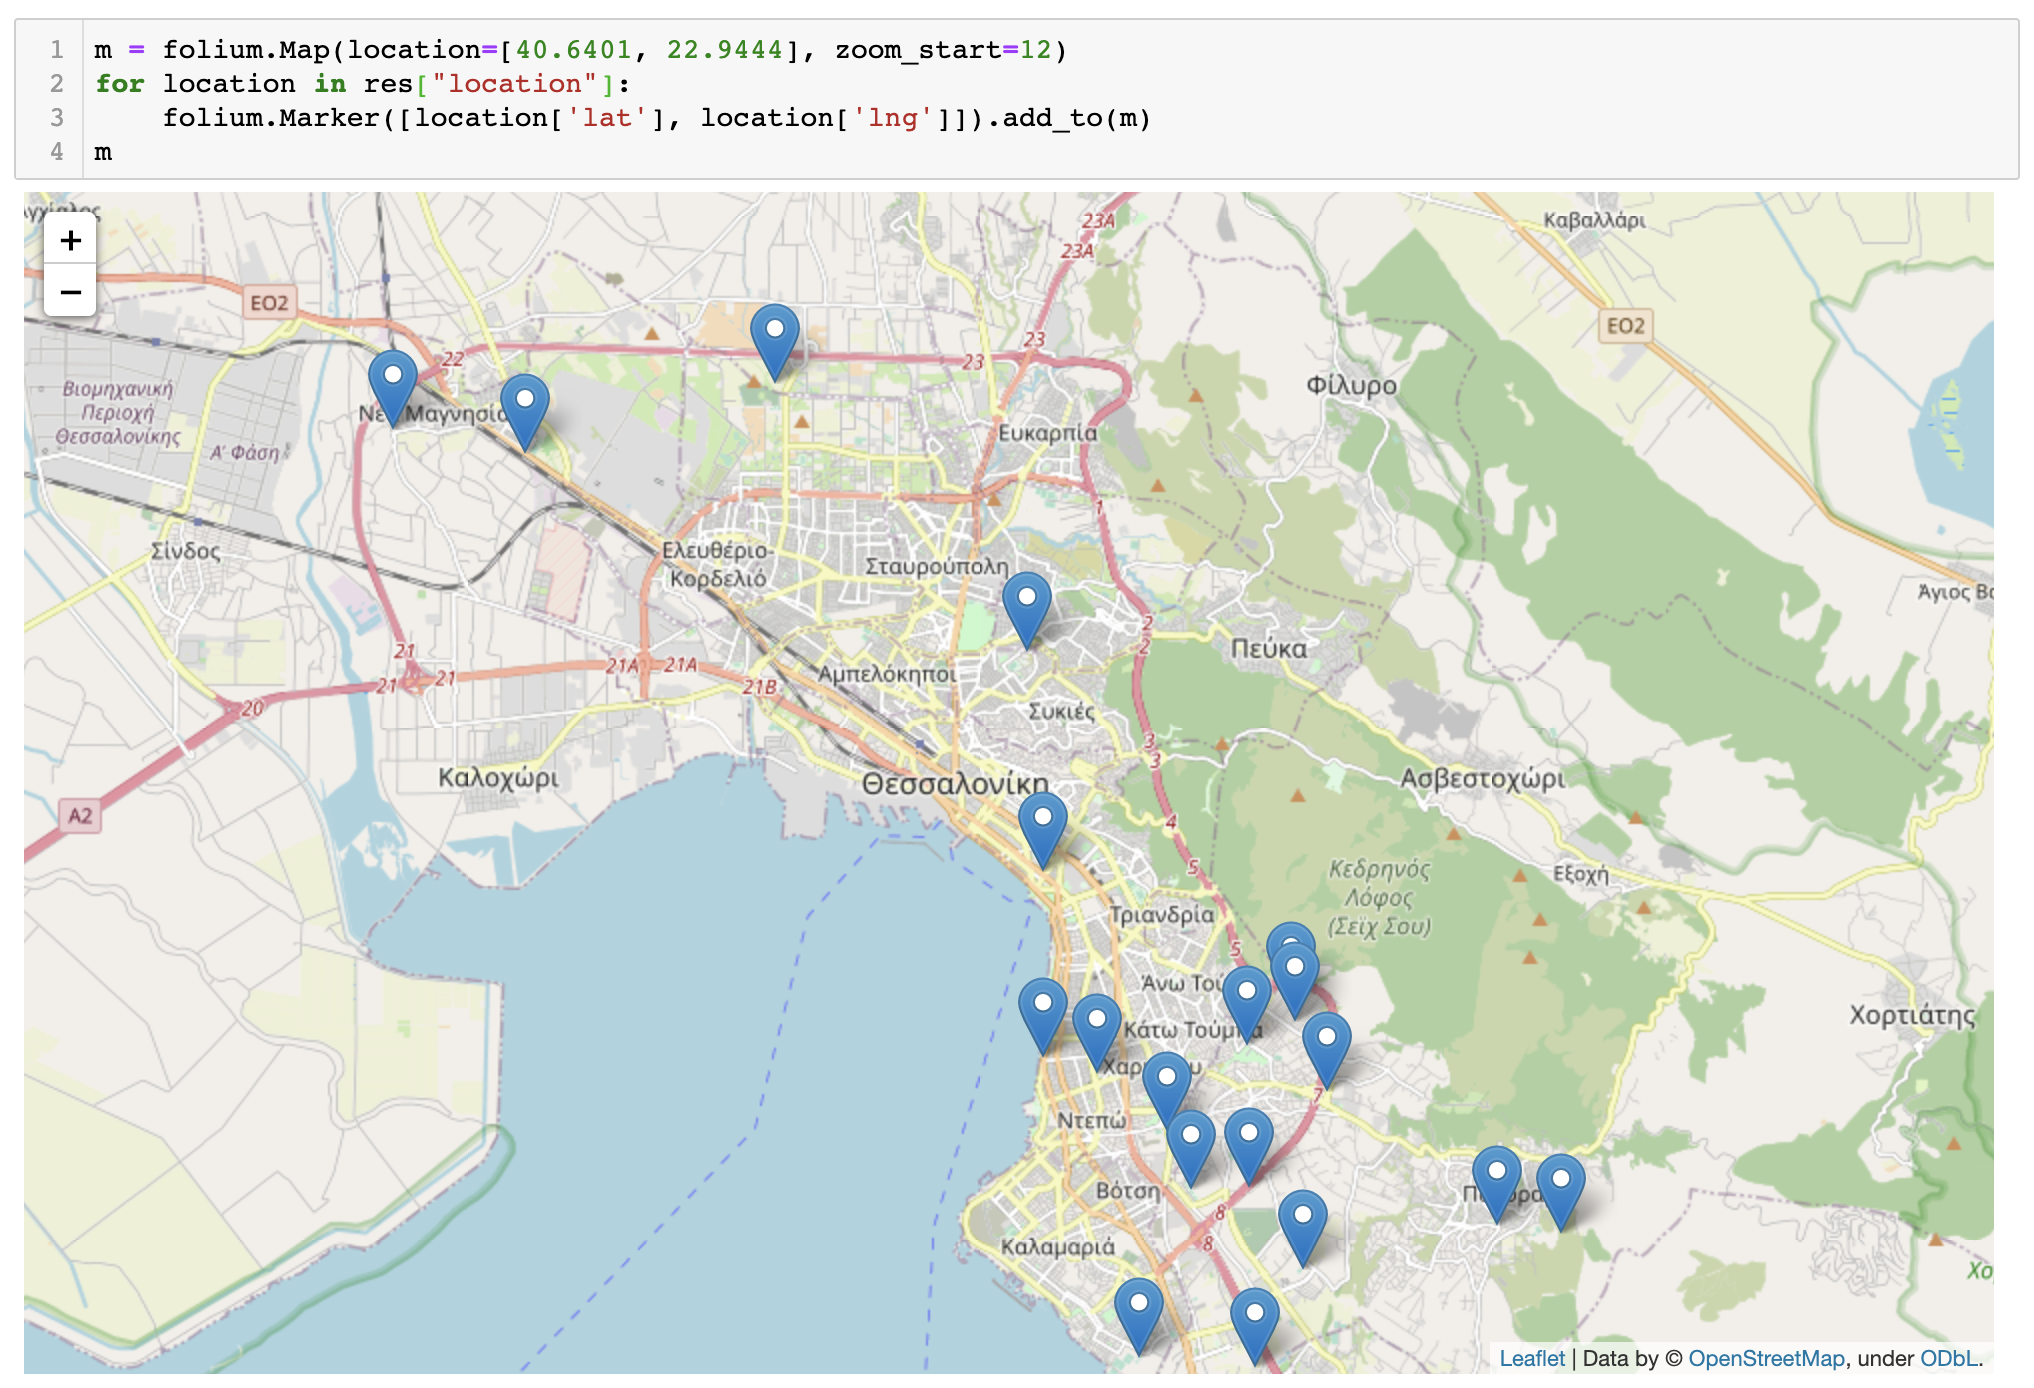
\includegraphics[scale=0.3]{map.png}}
\end{figure}

\end{enumerate}

\section{Results}
The resulting map that we ended up with after the analysis of the data, makes it obvious that some parts of the city have a greater need for sports facilities than others.

\begin{figure}[htbp]
\centerline{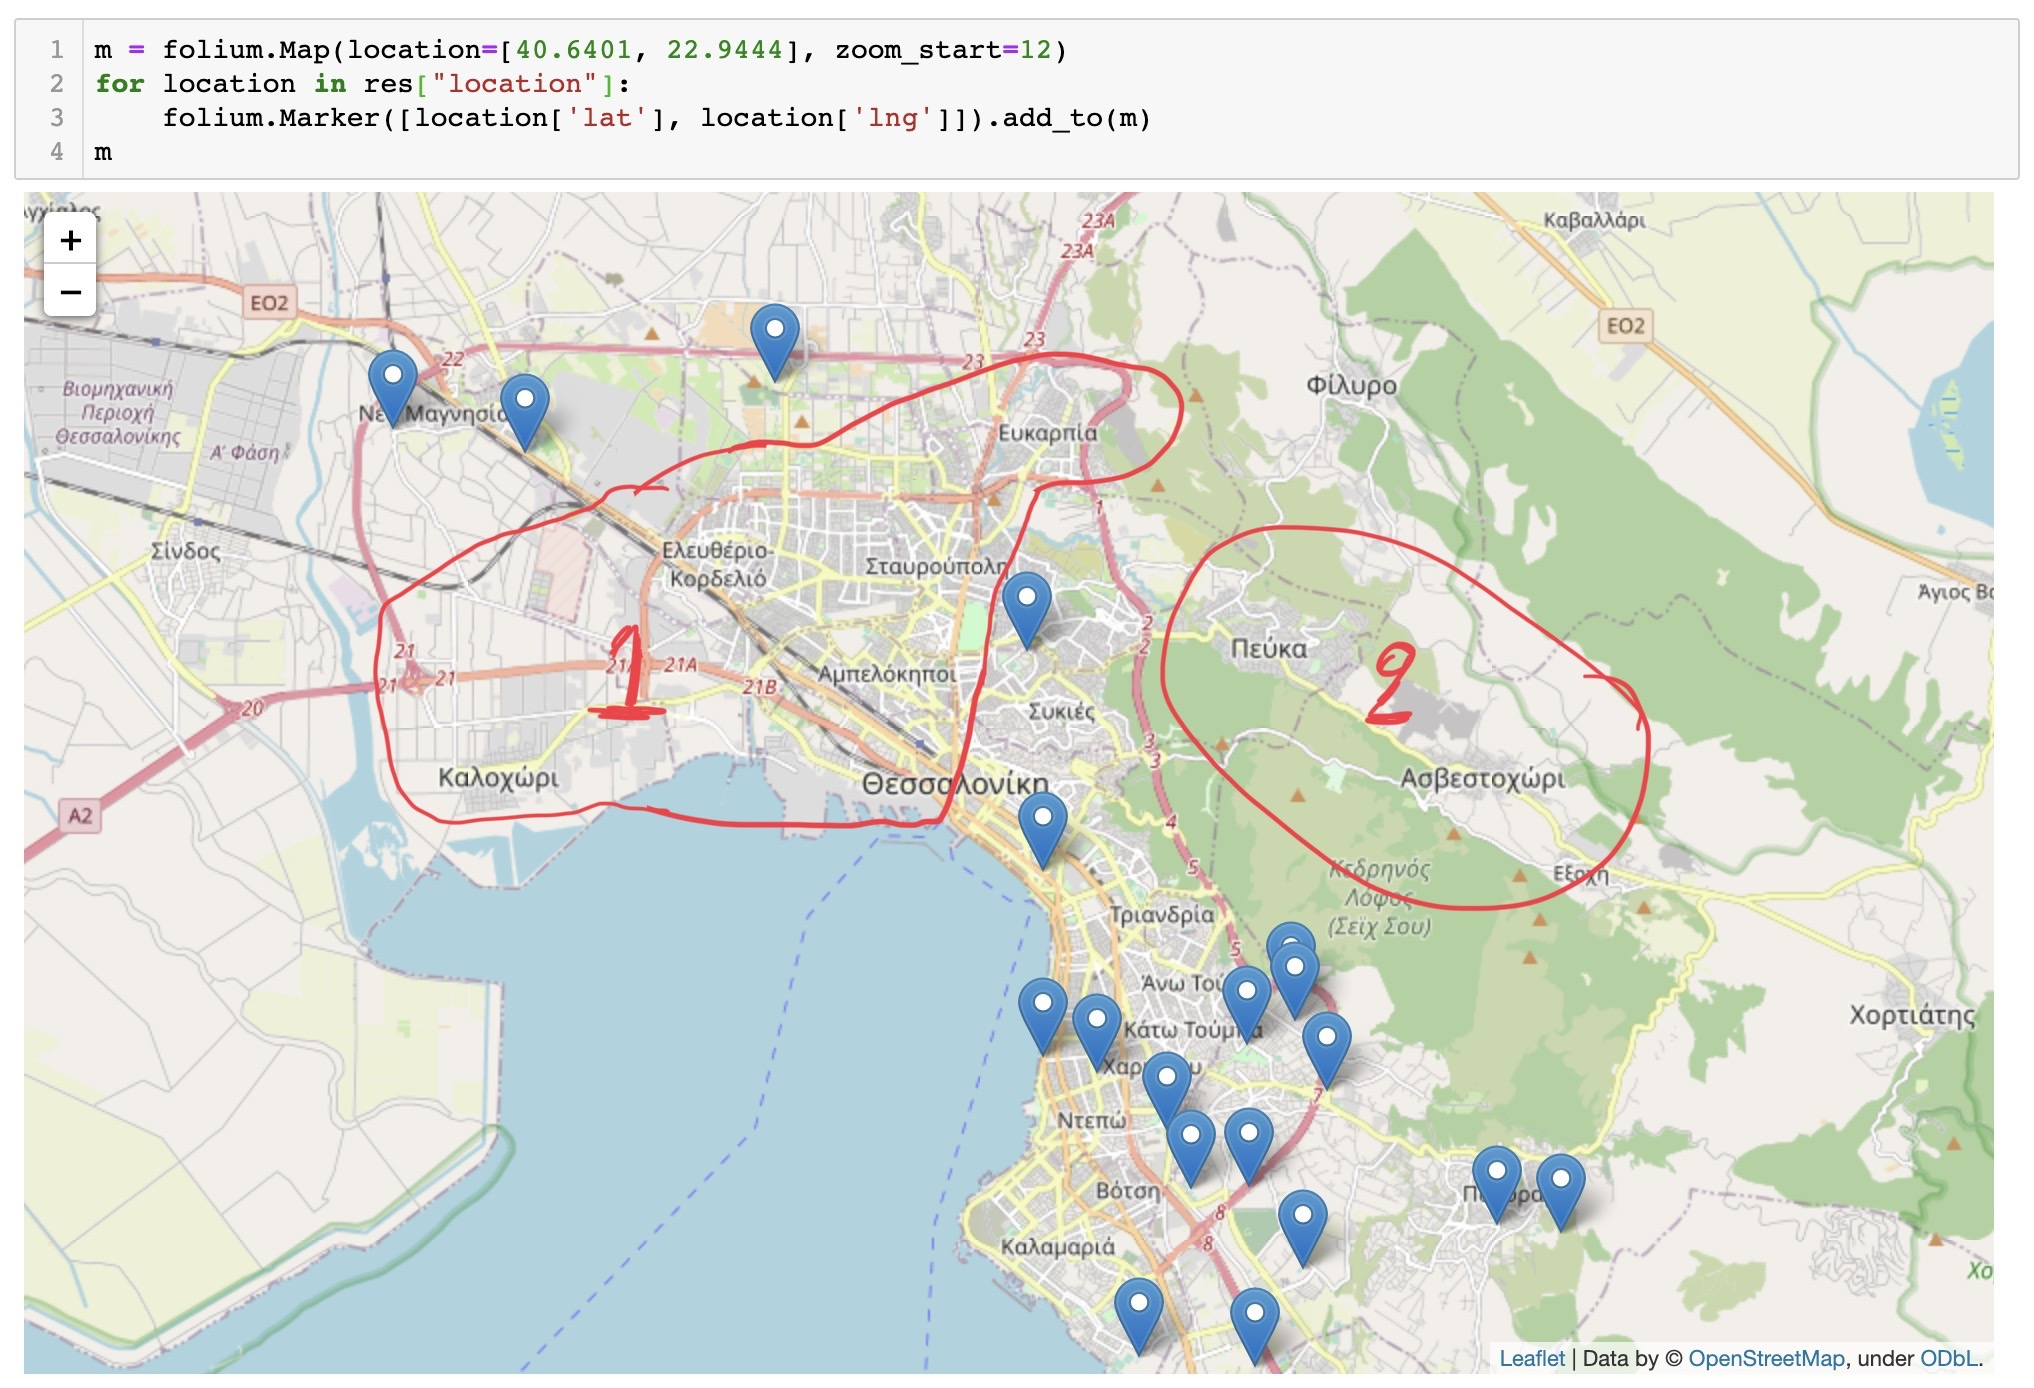
\includegraphics[scale=0.2]{map.JPG}}
\end{figure}

As we can see, although areas 1 and 2 in the map are quite central, they have zero sports centers. Therefore, a new related business in the area would be likely to be profitable, as there will be great demand for its services. Also, the Municipality of Thessaloniki could consider building open courts, accessible to everyone.

\pagebreak

\section{Discussion}
Even though the analysis came to a clear result, it could have been even more meaningful had there been enough data for the area. Unfortunately, lots of sports facilities were not identified by the Foursquare API. Also, not a single one of them had statistics about people that have visited the place, reviews, and rankings, which would have made it possible to classify "more complete" sports centers separately from simple courts. 

\section{Conclusion}
The outcome of this analysis suggests two big areas of the city that would support investment in the field of Sports Centers. Although there were some setbacks, mostly concerning the lack of detailed and complete data, the Foursquare API was still very helpful and allowed for us to get a resulting map making it obvious to the analyst where the courts should be built.


\end{document}
